\chapter{Dasar Teori}
\label{chap: dasarTeori}

Pada bab ini akan dijelaskan dasar-dasar teori mengenai CodeIgniter, AngularJS, dan Twitter Bootstrap.

\section{CodeIgniter}
\label{sec: codeigniter}

CodeIgniter\cite{ciDocs} merupakan sebuah \textit{framework} bagi \textit{programmer} yang ingin membuat sebuah \textit{web} dengan menggunakan bahasa PHP. Penggunaan CodeIgniter sendiri mempunyai tujuan mempercepat pengembangan proyek-proyek bersangkutan jika dibandingkan dengan menuliskan kode dari awal. Tujuan tersebut diwujudkan dengan tersedianya \textit{library} berisi \textit{task} yang biasa dibutuhkan dalam pengembangan \textit{program}, dibarengi dengan antarmuka yang sederhana serta struktur logika khusus untuk mengakses \textit{library} tersebut. Dengan begitu dapat disimpulkan bahwa CodeIgniter membuat pemrogram fokus pada kreativitas pembuatan \textit{program} dengan meminimalkan jumlah kode yang dituliskan.

\subsection{Flowchart Aplikasi CodeIgniter}
\label{sub: FlowAppCI}

Pada Gambar \ref{fig:flowchartCI} adalah \textit{flowchart} aliran data pada CodeIgniter.
\begin{figure}[H]
	\centering
	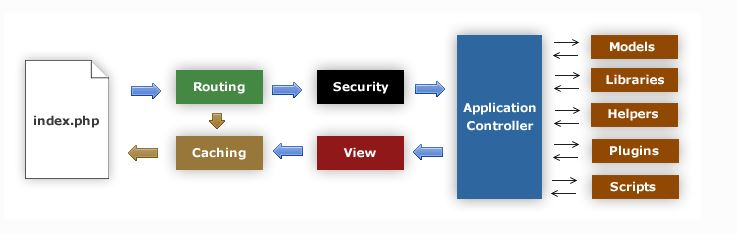
\includegraphics[scale=0.75]{Gambar/flowChartCI}
	\caption{Flowchart CodeIgniter}
	\label{fig:flowchartCI}
\end{figure}

Keterangan Gambar \ref{fig:flowchartCI}
\begin{enumerate}
	\item Index.php berfungsi sebagai pengontrol utama, yang menginisialisasikan sumber-sumber yang diperlukan untuk menjalankan CodeIgniter.
	\item \textit{Routing / Router} akan memeriksa permintaan HTTP untuk menentukan apa yang harus dilakukan selanjutnya
	\item Jika terdapat \textit{cache}, maka \textit{cache} tersebut akan dikirim langsung ke \textit{browser} dengan menjalankan sistem eksekusi \textit{normal}.
	\item  HTTP \textit{request} dan data yang diserahkan oleh \textit{user} akan disaring terlebih dahulu oleh bagian keamanan(\textit{security}) dari CodeIgniter, yang dijalankan sebelum \textit{controller} dari aplikasi diisi.
	\item \textit{Application Controller} akan mengambil isi dari \textit{model, libraries, helpers, plugins, scripts}, dan sumber lain yang diperlukan untuk menjalankan perintah-perintah spesifik.
	\item Kemudian \textit{View} akan diterjemahkan dari \textit{Application Controller} dan dikirim ke \textit{web browser} untuk kemudian ditampilkan. Jika pada \textit{view} akhir terdapat \textit{file cache}, maka \textit{view} tersebut akan terlebih dahulu dilakukan fungsi \textit{cached} sehingga permintaan berikutnya dapat dilayani.
\end{enumerate}

\subsection{Model-View-Controller}
\label{sub: MVC}

CodeIgniter menggunakan dasar pola pengembangan \textit{Model-View-Controller}(MVC). Pola pengembangan MVC ini merupakan suatu pendekatan yang memisahkan antara pengerjaan logika dan tampilan dari aplikasi.

MVC sendiri terdiri dari 3 bagian, yaitu:
\begin{enumerate}
	\item \textit{Model} merepresentasikan struktur data. Secara khusus, \textit{model} merupakan kelas yang membantu menangani kueri-kueri sql seperti \textit{insert, update,} dan \textit{delete} pada basis data.
	\item \textit{View} merepresentasikan informasi yang ditunjukkan kepada pengguna. Sebuah \textit{view} umumnya berbentuk \textit{web page}, tetapi dalam CodeIgniter \textit{view} bisa berbentuk \textit{header, footer,} dan berbagai jenis \textit{page} lainnya.
	\item \textit{Controller} berfungsi sebagai perantara antara \textit{Model}, \textit{View}, dan sumber daya lain yang diperlukan untuk memproses HTTP \textit{request} dan menghasilkan halaman \textit{web}.
\end{enumerate}

\subsection{Controller}
\label{sub: controller}

	\textit{Controller} merupakan sebuah kelas sederhana dengan penerapan seperti URL. Seperti kelas pada umumnya, ketika nama kelas dari \textit{controller} dan nama kelas dari \textit{file controller} tersebut cocok, maka kelas dapat dijalankan dengan baik. Nama kelas suatu \textit{controller} dikatakan sah jika diawali dengan huruf besar. Untuk lebih jelasnya, perhatikan kode di bawah ini:
\begin{lstlisting}[caption={CI Controller},label={CIcontroller}]
<?php
class Blog extends CI_Controller{
	
	public function index{
		echo 'Hello World';
	}
}
\end{lstlisting}

	Nama \textit{file} pada kode Listing \ref{CIcontroller} di atas haruslah  "Blog.php" dengan B besar dan disimpan pada \textit{application/controllers} sehingga URL dapat berjalan dengan baik.
	
\subsubsection{Method}
\label{subsub: method}

	\textit{Method} merupakan nama fungsi dari suatu kelas. Nama \textit{method} pada Listing \ref{CIcontroller} adalah "index()". \textit{Method} bernama "index" akan selalu dijalankan jika tidak ada arahan ke metode pada URL. Cara lain untuk menjalankan \textit{method} pada kode subbab \ref{sub: controller} adalah \url{example.com/index.php/blog/index/} dimana bagian terakhir adalah nama \textit{method} yang ingin dijalankan.
	
	
	\begin{lstlisting}[caption=CI Controller Method]
<?php
class Products extends CI_Controller{

	public function shoes($sandals, $id){
		echo $sandas;
		echo $id;
	}
}
	\end{lstlisting}
	
	Jika \textit{method} yang dituju memiliki parameter, diperlukan tambahan pada URL pemanggilannya. Sebagai contoh, pemanggilan \textit{method}	pada kode di atas dilakukan dengan URL \url{example.com/index.php/products/shoes/sandals/123} dimana "sandals" dan "123" merupakan isi dari \textit{parameter 1} dan 2 dari \textit{method} "shoes".
	
\subsubsection{Mendefinisikan Controller Default}
\label{subsub: defaulController}

	CodeIgniter dapat menjalankan \textit{default controller} sehingga tidak diperlukannya penulisan URL yang lengkap untuk pemanggilan, melainkan \textit{controller} dapat dipanggil secara otomatis dengan URL \url{example.com} saja. Namun, untuk dapat menjalankan fungsi ini, diperlukan sedikit pengaturan pada \textit{file} "application/config/routes.php" yaitu perubahan variabel yang ditunjukkan kode di bawah ini:
	
	\begin{lstlisting}[caption= Default Controller]
	$route['default_controller'] = 'blog';
	\end{lstlisting}
	
	"blog" merupakan nama \textit{file} \textit{controller} yang telah dibuat pada direktori "application/controllers/". Setelah pengaturan tersebut, maka pengguna bisa menjalankan aplikasi tanpa URL yang terspesifikasi menjalankan \textit{controller}.
	
	\subsection{Views}
	\label{sub: views}
	
	Sebuah \textit{views} merupakan bagian yang mengatur tampilan aplikasi yang akan ditunjukkan kepada pengguna. \textit{Views} meliputi \textit{footer, header, sidebar,} dll.
	Pada CodeIgniter, \textit{Views} tidak dapat dijalankan secara langsung dari URL, tapi \textit{views} harus dijalankan melalui file \textit{controller} yang ada. Hal ini dilakukan guna memudahkan \textit{programmer} dan mewujudkan \textit{framework MVC} pada CodeIgniter.
	
	\subsubsection{Pembuatan Views}
	\label{subsub: pembuatanView}
	
	Pembuatan \textit{file view} pada dasarnya sama seperti pembuatan \textit{file} berbasis PHP. Berikut ini merupakan salah satu contoh kode sebuah \textit{file view} sederhana.
	
	\begin{lstlisting}[caption={File View}, label={fileView}]
<html>
<head>
	<title> My Blog </title>
</head>
<body>
	<h1> Welcome to my Blog</h1>
</body>
</html>
	\end{lstlisting}
	
	Setelah selesai membuat \textit{file view} yang diinginkan, maka penyimpanan \textit{file} tersebut harus diletakkan di direktori "application/views/". Nama file pada view tidak diatur huruf besar maupun huruf kecil. Pada Listing \ref{fileView}, file disimpan dengan nama "blogview".
	
	\subsubsection{Menjalankan View}
	\label{subsub: menjalankanView}
	
	Menjalankan \textit{view} pada CodeIgniter dilakukan di \textit{file controller}. Listing di bawah ini menunjukkan kode yang harus ditulis di dalam \textit{method controller}.
	
	\begin{lstlisting}[caption={Pemanggilan View}, label={panggilView}]
<?php
class Blog extends CI_Controller{
	
	public function index(){
		$this->load->view('blogview');
	}
}
	\end{lstlisting}
	
	Listing \ref{panggilView} merupakan listing untuk memanggil view yang dibuat pada Listing \ref{fileView}, dimana "blogview" merupakan nama file view yang diinginkan.
	
	\subsection{Models}
	\label{sub: models}
	
	\textit{Model} merupakan \textit{file} berbasis PHP yang didesain sebagai penghubung aplikasi dengan basis data. \textit{Model} berfungsi menjalankan kueri-kueri sql seperti \textit{insert, update, delete, select,} dll.
	Pada CodeIgniter terdapat fungsi \textit{query builder} yang memudahkan \textit {programmer} dalam membuat kueri. Berikut ini adalah contoh penggunaan \textit{query builder} untuk kueri sql \textit{insert} dan \textit{update}.
	
	\begin{lstlisting}[caption={Query Builder Insert dan Update}, label={QueriBuild}]
public function insert_entry(){
	$this->title	= $_POST['title'];
	$this->content	= $_POST['content'];
	$this->date	= time();
	
	$this->db->insert('entries',$this);
}

public function update_entry(){
	$this->title	= $_POST['title'];
	$this->content	= $_POST['content'];
	$this->date	= time();
	
	$this->db->update('entries',$this, array('id') => $POST['id']);
}
	\end{lstlisting}
	
	Pada Listing \ref{QueriBuild}, merupakan contoh penggunaan Query Builder dari Codeigniter. Pada method insert terdapat "\$this->title = \$\_POST['title'];" yang berarti bahwa variabel "title" akan mengambil masukan dari \textit{form view} yang memiliki variable "name = title". Setelah itu variabel akan dimasukkan ke Query Builder pada baris terakhir dari \textit{method insert} dan \textit{update}.
	
	Penamaan \textit{file} pada \textit{model} tidak memiliki aturan baku seperti pada \textit{file controller}. \textit{File model} pada Listing \ref{QueriBuild} disimpan dengan nama "blog.php".
	
	\subsubsection{Menjalankan Model}
	\label{subsub: menjalankanModel}
		
	Sama seperti menjalankan \textit{file view}, \textit{model} pun tidak bisa dijalankan secara langsung menggunakan URL. Untuk menjalankan \textit{model} perlu dilakukan pemanggilan pada \textit{controller}.
	
	\begin{lstlisting}[caption={Pemanggilan File Model}, label={panggilModel}]
class Blog_controller extends CI_Controller {

	public function blog(){
		$this->load->model('blog');
		$data['query'] = $this->blog->get_last_ten_entries();
		$this->load->view('blog',$data);
	}
}
	\end{lstlisting}
	
	Listing \ref{panggilModel} di atas menunjukkan bahwa \textit{file controller} melakukan pemanggilan \textit{model} yang diikuti dengan inisialisasi \textit{array data} dari basis data yang dimasukkan ke pemanggilan \textit{view}, dimana "blog" pada baris 4 adalah nama \textit{file model}, dan "blog" pada baris 6 adalah nama dari \textit{file view} yang diinginkan.
	
	\subsection{Helper}
	\label{sub: helper}
	
	\textit{Helper} merupakan kelas yang membantu \textit{programmer} dalam menjalankan \textit{task}. CodeIgniter memiliki banyak kelas \textit{helper}, seperti \textit{URL Helper} yang membantu dalam membuat \textit{link}, \textit{Form Helper} yang membantu dalam pembuatan elemen-elemen di dalam form, \textit{Text Helper} yang membantu dalam menjalankan berbagai \textit{text formatting routines}, \textit{Cookies Helper} yang membantu dalam mengatur dan membaca \textit{cookies} yang ada, dll. \textit{Helper} pada CodeIgniter umumnya ada pada direktori "application/helpers directory" atau "system/helpers". 
	
	\subsubsection{Menjalankan Helper}
	\label{subsub: menjalnkanHelper}
	
	Cara menjalankan \textit{helper} pada CodeIgniter cukup dengan menambahkan kode di dalam \textit{file Helper} atau \textit{view}.
	
	\begin{lstlisting}[caption="Kode Helper", label={jalanHelper}]
$this->load->helper('name');
	\end{lstlisting}
	
	Penulisan "name" pada Listing \ref{jalanHelper} diatas diisi dengan \textit{part helper} yang diinginkan. Contoh jika pada aplikasi perlu \textit{URL Helper} maka "name" diganti dengan "url". Helper juga dapat dijalankan secara otomatis dengan cara mengisi variable 'helper' pada \textit{file autoload} yang berada di direktori "application/config/autoload.php".
	
	\subsection{Basis data}
	\label{sub: database}
	
	\subsubsection{Menyambungkan ke Basis Data}
	\label{subsub: connectDatabase}
	
	Perlu diingat bahwa kelas \textit{model} tidak menjalankan basis data secara otomatis. Untuk membuat aplikasi terkoneksi dengan basis data, diperlukan beberapa tambahan kode pada \textit{file model} atau \textit{file controller}.
	CodeIgniter memiliki fitur \textit{automatically connecting} yang membuat seluruh aplikasi tersambung dengan basis data pada setiap \textit{page load}. untuk mengaktifkan fitur ini cukup mengetikkan "database" pada variabel autoload['libraries'] di "application/config/autoload.php" seperti kode dibawah ini.
	
	\begin{lstlisting}
$autoload['libraries'] =array('database');
	\end{lstlisting}
	
	Selain \textit{autoload}, CodeIgniter juga mendukung koneksi ke basis data dengan cara manual, dengan cara menambahkan "\$this->load->database();" pada \textit{method} atau kelas basis data ingin dijalankan.
	
	\subsection{Konfigurasi Basis Data}
	\label{sub: databaseConf}
	
	Konfigurasi basis data pada CodeIgniter disimpan dengan cara \textit{multi-dimensional array}.
	
	\begin{lstlisting}[caption=Array Basis Data, label=isiBasDat]
$db['default'] = array(
		'dsn'		=> '',
		'hostname'	=> 'localhost',
		'usernmae'	=> 'root',
		'password'	=> '',
		'database'	=> 'database_name',
		'dbdriver'	=> 'mysqli',
		'dbprefix'	=> '',
		'pconnect'	=> TRUE,
		'db_debug'	=> TRUE,
		'cache_on'	=> FALSE,
		'cachedir'	=> '',
		'char_set'	=> 'utf8',
		'dbcollat'	=> 'utf_general_ci',
		'swap_pre'	=> '',
		'encrypt'	=> FALSE,
		'compress'	=> FALSE,
		'striction'	=> FALSE,
		'failover'	=> array()
	);
	\end{lstlisting}
	\pagebreak
	Keterangan Listing \ref{isiBasDat}:
	\begin{center}
	\begin{tabular}{| m{5cm} | m{10cm} |}
		\hline
		Nama Konfigurasi & Deskripsi\\
		\hline
		dsn & membuat koneksi string  (\textit{an all-in-one configuration sequence})\\
		\hline
		hostname & nama host dari server basis data yang dipakai (umumnya bernama "localhost").\\
		\hline
		username & username yang dipakai untuk menyambungkan basis data\\
		\hline
		password & password yang cocok dengan username yang dipakai untuk menyambungkan basis data\\
		\hline
		database & nama basis data yang ingin di sambungkan\\
		\hline
		dbdriver & tipe basis data (mysqli, postgre, odbc, dll). Perlu ditulis dengan huruf kecil secara spesifik.\\
		\hline
		dbprefix & dbprefix tidak harus terisi, berguna untuk menambahkan awalan nama tabel pada saat dijalankan \textit{query builder}.\\
		\hline
		pconnect & berisi TRUE atau FALSE untuk perlunya koneksi yang tetap\\
		\hline
		db\_debug & berisi TRUE atau FALSE untuk perlunya menampilkan error dari basis data\\
		\hline
		cache\_on & berisi TRUE atau FALSE untuk diperbolehkannya database query caching\\
		\hline
		cachedir & server path yang mutlak untuk direktori database query cache\\
		\hline
		char\_set & set karakter yang digunakan untuk komunikasi dengan basis data\\
		\hline
		dbcollat & pemeriksaan karakter yang digunakan dalam berkomunikasi dengan basis data (hanya dipakai di driver 'mysqli' dan 'mysql').\\
		\hline
		swap\_pre & sebuah tabel default yang harus bertukar dengan dbprefix.\\
		\hline
		schema & skema basis data yang nilai defaultnya adalah 'public'. Digunakan untuk driver PostgreSQL and ODBC.\\
		\hline
		encrypt &  berisi TRUE atau FALSE perlu tidaknya memakai koneksi yang ter-enkripsi.\\
		\hline
		compress & perlu tidaknya memakai client compression (hanya untuk MYSQl)\\
		\hline
		stricton &  berisi TRUE atau FALSE untuk perlu tidaknya memakai koneksi "Strict Mode" \\
		\hline
		port & nomor port dari basis data. Untuk menggunakannya diperlukan penambahan di config array database.\\
		\hline
	\end{tabular}
\end{center}
	
\section{AngularJS}
\label{sec: angularJS}

AngularJS\cite{AngularJSDocs} merupakan sebuah \textit{framework} terstruktur yang digunakan untuk aplikasi \textit{web} yang bersifat dinamis. Hal tersebut memungkinkan \textit{programmer} untuk mempergunakan HTML sebagai \textit{template} bahasa pemrograman dan memperluas sintaks HTML agar dapat mengekspresikan komponen aplikasi dengan jelas dan ringkas. Sifat AngularJS yang mengikat data dan mempunyai injeksi ketergantungan (\textit{Dependency Injection}) yang berfungsi agar suatu kelas tidak terikat dengan kelas lain, juga akan menghilangkan banyak kode yang seharusnya dituliskan oleh \textit{programmer}, dan semua itu terjadi pada \textit{browser} sehingga dapat disimpulkan bahwa AngularJS merupakan pasangan yang sangat ideal bagi penggunaan teknologi server. 
Dalam pembuatannya, ketidakcocokkan halaman statik dan dinamik biasanya diselesaikan dengan pendekatan sebagai berikut:
\begin{enumerate}
	\item \textit{Library}: merupakan sebuah koleksi dari berbagai macam fungsi yang berguna dalam pembuatan aplikasi \textit{web}, contoh: JQuery.
	\item \textit{Frameworks}: merupakan suatu implementasi dari sebuah aplikasi \textit{web} yang menempatkan kode yang dituliskan secara detail. \textit{Framework} akan berperan melakukan pemanggilan ke kode yang dituliskan \textit{programmer} ketika aplikasi membutuhkan sesuatu yang spesifik, contoh: durandal(\textit{light-weight javascript framework}), ember(\textit{open-source javascript framework}), dll.
\end{enumerate}

Dalam pembentukannya, AngularJS memiliki pendekatan yang berbeda. AngularJS mengajarkan \textit{browser} sintaks baru yang disebut \textit{directives}. Contoh \textit{directives} adalah:
\begin{enumerate}
	\item Keterikatan data di dalam \{\{\}\};
	\item Dukungan untuk \textit{Form} dan \textit{Form Validation}
	\item Pengelompokkan HTMl menjadi komponen - komponen yang dapat dipakai kembali.
\end{enumerate}

\subsection{Gambaran Konseptual}
\label{sub: gambaranKonsep}
	Berikut ini adalah beberapa bagian-bagian terpenting dalam AngularJS.
	\begin{center}
		\begin{tabular}{| m{5cm} | m{10cm} |}
			\hline
			Konsep & Deskripsi \\
			\hline
			Template & HTML dengan tambahan \textit{markup} \\
			\hline
			Directives & Pengembangan HTML dengan atribut dan elemen yang dibuat khusus \\
			\hline
			Model & Data yang ditunjukan kepada pengguna pada tampilan dan bagaimana penguna berinteraksi \\
			\hline
			Scope & Konteks dimana model disimpan sehingga \textit{controller, directives} dan \textit{expression} dapat mengaksesnya \\
			\hline
			Expression & Mengakses variabel dan fungsi dari \textit{scope} \\
			\hline
			Compiler & Menguraikan \textit{template, directives,} dan \textit{expression} \\
			\hline
			Filter & Mengatur nilai dari sebuah \textit{expression} untuk di tunjukkan kepada pengguna \\
			\hline
			View & Apa yang akan dilihat oleh pengguna\\
			\hline
			Data Binding & Menyelaraskan data yang ada pada \textit{model} dan view \\
			\hline
			Controller & Mengatur logika dibalik tampilan \\
			\hline
			Dependency Injection & Membuat dan menyambungkan objek dan fungsi \\
			\hline
			Injector & Tempat penyimpanan \textit{dependency injection} \\
			\hline
			Module & Tempat penyimpanan untuk bagian-bagian yang berbeda dalam sebuah aplikasi, yang mencakup: \textit{controllers, services, filters, directives} yang mengkonfigurasikan \textit{injector} \\
			\hline
			Services & Logika bisnis independen dari \textit{views} yang bisa dipakai kembali  \\
			\hline
			\end{tabular}
		\end{center}
		
\subsection{Directives}
\label{sub: directives}

	\textit{Directives} merupakan penanda pada \textit{DOM (Document Object Mode) elements} (seperti attribut, nama, \textit{comment},  dan kelas CSS) yang memberitahukan kepada \textit{AngularJS HTML compiler}\footnote{memperbolehkan pengembang untuk mengajarkan browser syntaks HTML baru}, sehingga dapat melampirkan perilaku yang diinginkan kepada \textit{DOM element} (contohnya memakai \textit{event listener}), atau bahkan mengubah \textit{DOM element} yang dituju beserta dengan peranakannya.
	
	AngularJS menyediakan sekumpulan \textit{directives built-in} seperti yang akan dijelaskan selanjutnya.
	
	\subsubsection{ng-Model}
	ng-Model adalah suatu \textit{directives} yang dapat digunakan pada \textit{form control} seperti \textit{input, select, textarea}, dan \textit{form control} unik lainnya untuk mengikat data ke \textit{scope property (\$scope)} dengan menggunakan ngModelController (kelas yang menyediakan API (\textit{Application Programming Interface}) untuk ng-Model)
	
	\subsubsection{ng-Controller}
	ng-Controller adalah suatu \textit{directives} yang menambahkan suatu kelas \textit{controller} pada bagian \textit{view} dari aplikasi angularJS. ng-Controller inilah yang merupakan kelas kunci dari bagaimana AngularJS dapat menerapkan Model-View-Controller bersifat front-end (pada tampilan).

\subsection{Data Binding}
\label{sub: dataBinding}
	
	\textit{Data Binding} pada AngularJS merupakan penyelarasan data antara \textit{model} dan komponen-komponen \textit{view}. Ketika \textit{model} berubah, maka \textit{view} pun akan berubah, begitu juga dengan sebaliknya.
	
	\begin{figure}[H]
		\centering
		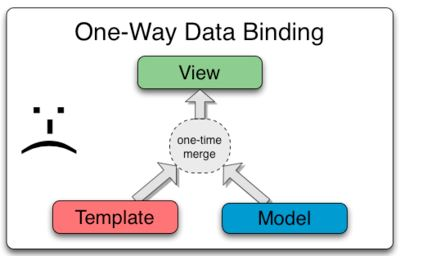
\includegraphics[scale=0.75]{Gambar/Dabin1}
		\caption{Data Binding Classical Templates System}
		\label{fig:dabin1}
	\end{figure}
	Pada gambar \ref{fig:dabin1} menjelaskan bahwa kebanyakan \textit{data binding} adalah proses satu arah. Hal itu dilakukan dengan menyatukan \textit{template} dan \textit{model} menjadi \textit{view}. Setelah penyatuan, pergantian pada \textit{model} tidak secara otomatis mengganti \textit{view} yang sudah ditampilkan.
	\begin{figure}[H]
		\centering
		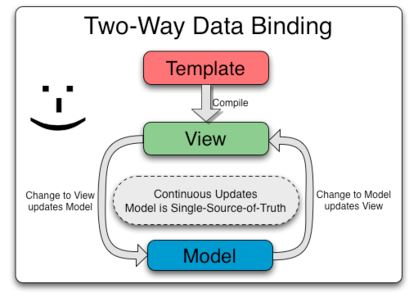
\includegraphics[scale=0.75]{Gambar/Dabin2}
		\caption{Data Binding pada Angular}
		\label{fig:dabin2}
	\end{figure}
	Pada gambar \ref{fig:dabin2} menjelaskan perbedaan yang diberikan oleh pelaksanaan \textit{data binding} pada AngularJS. Pertama, \textit{template} akan di \textit{compile} pada \textit{browser}. Hasil dari \textit{compile} tersebut adalah \textit{live view}. Pada tahap ini perubahan yang terjadi di \textit{view} akan disampaikan kepada \textit{model}, dan perubahan yang terjadi pada \textit{model} akan mengubah \textit{view}.
	
	Karena \textit{view} merupakan proyeksi dari \textit{model}, menyebabkan \textit{controller} benar-benar terpisahkan dari \textit{view} tanpa disadari. Hal ini mempermudah pengujian \textit{controller}, karena terisolasi tanpa adanya \textit{view} dan DOM (\textit{browser dependency}).
	
\subsection{Model-View-Controller(MVC)}
\label{sub: mvcAngular}

	AngularJS\cite{green2013angularjs} juga merupakan salah satu \textit{framework} yang menggunakan  \textit{Model-View-Controller} sebagai patokan desain aplikasi. Walaupun AngularJS mempunyai banyak flexibilitas dalam membangun aplikasi, tetapi akan ada beberapa hal yang selalu dijumpai dalam mendesain sebuah aplikasi, diantaranya:
	\begin{itemize}
		\item Sebuah \textit{model} selalu menampung data yang merepresentasikan keadaan aplikasi.
		\item \textit{Views} yang menyajikan data tersebut.
		\item \textit{Controller} yang akan selalu mengatur hubungan antara \textit{model} dan \textit{views}.
	\end{itemize}
	
	Model dibuat dengan menggunakan atribut berupa objek atau konten-konten primitif yang dapat menyimpan data. Berikut adalah salah satu contoh praktis dalam pembuatan \textit{model}:
\begin{lstlisting}[caption= Model berupa variabel]
var someText = 'You have started your journey.'
\end{lstlisting}
	Setelah itu untuk menampilkannya maka perlu dibuat \textit{view} dari data \textit{model} "someText" diatas dengan cara:
\begin{lstlisting}[caption= Menampilkan model]
<p> {{someText}} </p>
\end{lstlisting}
	\textit{Syntax view} 2 kurung kurawal diatas disebut sebagai interlopasi (penyusupan), karena hal tersebut memasukkan konten baru ke dalam \textit{template} yang sudah ada.\\
	Sementara kelas \textit{controllers} berguna untuk memberitahu AngularJS tentang objek atau konten primitif mana dari \textit{model} yang akan dipakai dengan cara menetapkannya ke objek '\$scope ', objek '\$scope' tersebut kemudian akan diberikan kepada \textit{controller} seperti contoh berikut:
\begin{lstlisting}[caption= Controller , label= listController]
function TextController($scope){
	$scope.someText = someText;
}
\end{lstlisting}
	
	Berikut ini adalah contoh penggabungan fungsi \textit{model, view,} dan \textit{controller}:
\begin{lstlisting}[caption= Penyatuan model view controller , label=penyatuanCI]
<html>
<body ng-controller = "TextController">
	<p>{{someText}}</p>
	
	<script>
		src="https://ajax.googleapis.com/ajax/libs/angularjs/1.0.4/angular.min.js">
	</script>
	
	<script>
		function TextController($scope){
			$scope.someText = 'You have started your journey.';
		}
	</script>
</body>
</html>
\end{lstlisting}
	
	Hasil dari Listing \ref{penyatuanCI} diatas adalah tulisan "You have started your journey". Walaupun cara ini dapat dilakukan dengan mudah pada aplikasi sederhana seperti contoh diatas, tetapi untuk kebanyakan aplikasi sebaiknya dibuat objek \textit{model} untuk menyimpan \textit{data} yang ada. Untuk itu, daripada membuat \textit{model} seperti Listing \ref{listController}, akan lebih baik menggunakan kode:
\begin{lstlisting}[caption= Penyederhanaan controller]
var message= {};
message.someText = 'You have started your journey';
function TextController($scope){
	$scope.message = message;
}
\end{lstlisting}
	Yang kemudian akan dipanggil di \textit{template} dengan kode:
\begin{lstlisting}[caption= Pemanggilan variabel]
<p>{{message.someText}}</p>
\end{lstlisting}
	Perubahan yang dilakukan diatas berfungsi untuk mencegah perilaku tidak terduga yang dapat terjadi dari \textit{prototypal inheritance} dalam objek '\$scope'. Walaupun untuk sementara hal ini dapat berjalan dengan baik, tetapi cara yang benar dalam mendefinisikan sebuah \textit{controller} adalah dengan menggunakan sebuah kelas yang dinamakan \textit{module} yang menyediakan \textit{namespace} untuk bagian lain dari aplikasi berhubungan. Perubahan tersebut akan mengubah kode-kode pada listing diatas menjadi:
	\begin{lstlisting}[caption= Penyederhanaan MVC]
<html ng-app='myApp'>
<body ng-controller='TextController'>
	<p>{{someText.message}}</p>
	<script>
		src="https://ajax.googleapis.com/ajax/libs/angularjs/1.0.4/angular.min.js">
	</script>
	
	<script>
		var myAppModule = angular.module('myApp',[]);
		
		myAppModule.controller('TextController',
			function($scope){
			var someText = {};
			someText.message = 'You have started your journey';
			$scope.someText = someText;
		});
	</script>
</body>
</html>
	\end{lstlisting}
	Pada versi di atas, aplikasi memberi tahu elemen ng-app tentang nama dari modul yang dipakai di baris ke-9. Setelah itu pada baris ke-11 sampai baris ke-16 dilakukan pemanggilan objek AngularJS untuk membuat sebuah modul bernama myApp dan memberikan fungsi dari \textit{controller} untuk memanggil fungsi \textit{controller} dari modul.
	
\section{Twitter Bootstrap}
\label{sec: Bootrstrap}

\textit{Twitter Bootstrap}\cite{bootstrap} atau yang lebih dikenal dengan \textit{Bootstrap} adalah \textit{framework} HTML, CSS, dan JS terpopuler dalam hal pengembangan tampilan yang responsif \textit{mobile} pertama dalam hal aplikasi berbasis \textit{web}. 

\subsection{Grid System}
\label{sub: gridSystem}

\textit{Bootstrap} merupakan responsif \textit{mobile} pertama yang mempunyai sistem skala (\textit{grid system}). Sistem skala tersebut membagi layar perangkat menjadi 12 kolom yang berukuran sama, dimana besar ukuran masing-masing kolom mengikuti besar layar perangkat. Ketika layar semakin besar, maka ukuran masing-masing kolom pun akan semakin besar, begitu juga sebaliknya. Cara sistem skala \textit{Bootstrap} bekerja adalah:

\begin{enumerate}
	\item \textit{Rows} harus ditempatkan diantara \textit{.container(fixed-width)} atau \textit{.container-fluid (full-width)} untuk mendapatkan keselarasan ukuran
	\item \textit{Rows} dipergunakan untuk membuat grup kolom secara \textit{horizontal}.
	\item Konten tampilan harus berada diantara kelas \textit{columns} atau peranakan dari kelas \textit{columns}.
	\item Kelas-kelas yang telah ditetapkan seperti ".row" dan ".col-xs-4" dapat digunakan dengan segera untuk membentuk \textit{layout}.
	\item Kelas \textit{columns} membuat \textit{gutters} (jarak antara kolum konten) menggunakan kelas \textit{padding}.
	\item \textit{Grid columns} dibuat dengan menyesuaikan ke-12 kolom yang sudah disediakan. Contohnya jika ingin membuat 3 kolom sama rata, maka diperlukan 3 buah kelas ".col-xs-4".
	\item Jika ada lebih dari 12 kolom dalam 1 baris, maka kolom yang lebih tersebut akan dipindahkan ke baris baru sebagai satu kesatuan.
	\item Kelas \textit{grid} mempunyai fungsi untuk menyesuaikan ukuran sesuai dengan patokan ukuran yang sudah diberikan oleh \textit{bootstrap} atau lebih besar dari angka patokan yang ada. Oleh karena itu ketika sebuah kelas ".col-md-*" tidak memiliki kelas yang lebih besar darinya seperti kelas ".col-lg-*", maka kelas md akan mengambil alih pada saat aplikasi dijalankan di ukuran perangkat yang lebih besar. 
\end{enumerate}
	
\begin{figure}[H]
	\centering
	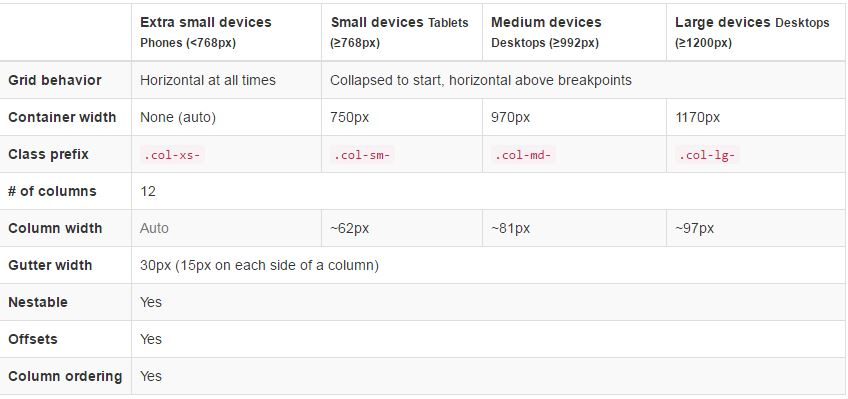
\includegraphics[scale=0.75]{Gambar/gridOption}
	\caption{Grid Option pada Bootstrap}
	\label{fig:gridOpt}
\end{figure}

\begin{figure}[H]
	\centering
	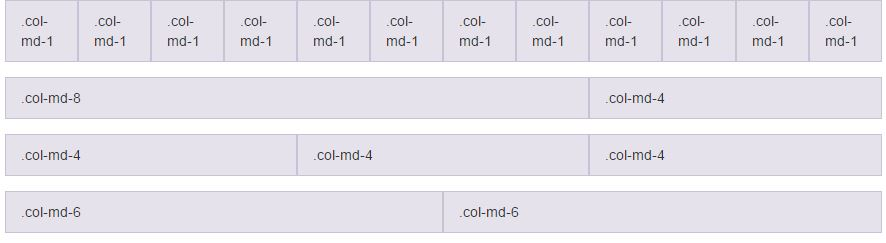
\includegraphics[scale=0.75]{Gambar/kolom}
	\caption{Contoh Pembagian Grid Columns}
	\label{fig:gridCol}
\end{figure}

\subsection{Form Class}
\label{sub: formClass}
	Masing-masing form akan memiliki bentuk otomatis yang diatur secara global. Dengan memakai kelas ".form-control", pengaturan ukuran dari kelas <input>, <textarea>, dan <select> akan otomatis memiliki variabel \textit{width} 100\% secara \textit{default}. Untuk mendapatkan jarak \textit{spacing} yang maksimal, \textit{Bootstrap} memiliki kelas ".form-group" yang membungkus kelas \textit{form} menjadi grup-grup.
	
\begin{lstlisting}[caption= Contoh penggunaan Twitter Bootstrap]
<form>
	<div class="form-group">
		<label for="exampleInputEmail1">Email Address</label>
		<input type="email" class="form-control" id="exampleInputEmail1" placeholder="Email">
	</div>
	<div>
		<label for=exampleInputPassword1">Password</label>
		<input type="password" class="form-control" id="exampleInputPassword1" placeholder="Password">
	</div>
	<div class="form-group">
		<label for="exampleInputFile">File</label>
		<input type="file" id="exampleInputFile">
		<p class="help-block"> Example block-level help text here.</p>
	</div>
	<div class="checkbox">
		<label>
			<input type="checkbox"> Check me out
		</label>
	</div>
	<button type="submit" class="btn bt-default">Submit</button>
</form>
\end{lstlisting}

\begin{figure}[H]
	\centering
	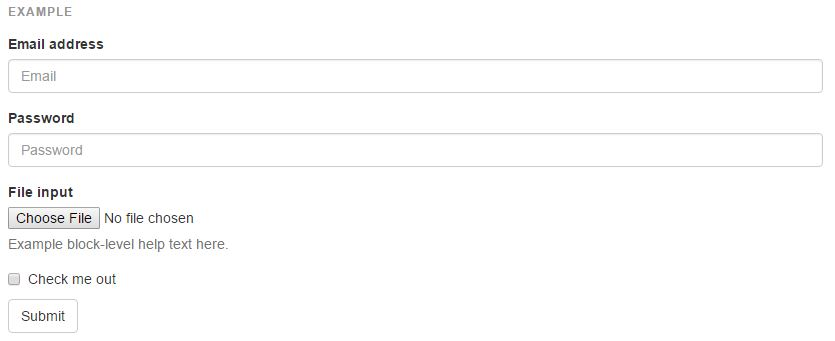
\includegraphics[scale=0.75]{Gambar/hasilForm}
	\caption{Contoh Hasil Pengggunaan Kelas Form}
	\label{fig:hasilForm}
\end{figure}